% ---------------------------------------------------------------
% Architecture
% MVP architecture in detail. Use multiple views (e.g. C4) and
% complementary diagrams. Describe how the design supports each ASR.
% Diagrams live in /model and are exported to PDF/PNG for inclusion here.
% ---------------------------------------------------------------
\section{Architecture}
\label{sec:arch}

The option selected in Section~\ref{sec:options} is realised as a modular-monolith API supported by two extracted event-driven processes, a small set of specialised datastores, and a single-page web client. This section describes that realisation using the C4 model (system context, containers, and components), then traces the dominant runtime flow and sets out how the structure satisfies each architecturally significant requirement (ASR). The figures are generated from the authoritative diagram sources under \texttt{model/artefacts/}; the full set, including the entity-relationship model and the remaining sequence diagrams, lives there. In practical terms, the architecture keeps the synchronous user-facing features inside the FastAPI API, while separating burst-heavy and failure-prone work, such as notification fan-out and scheduled visibility transitions, into the outbox relay and notification worker. This separation allows the MVP to remain simple to deploy and test, while still giving the system a credible path to scale or extract modules in the future.

\subsection{System Context (C4 Level 1)}

\begin{figure}[htbp]
  \centering
  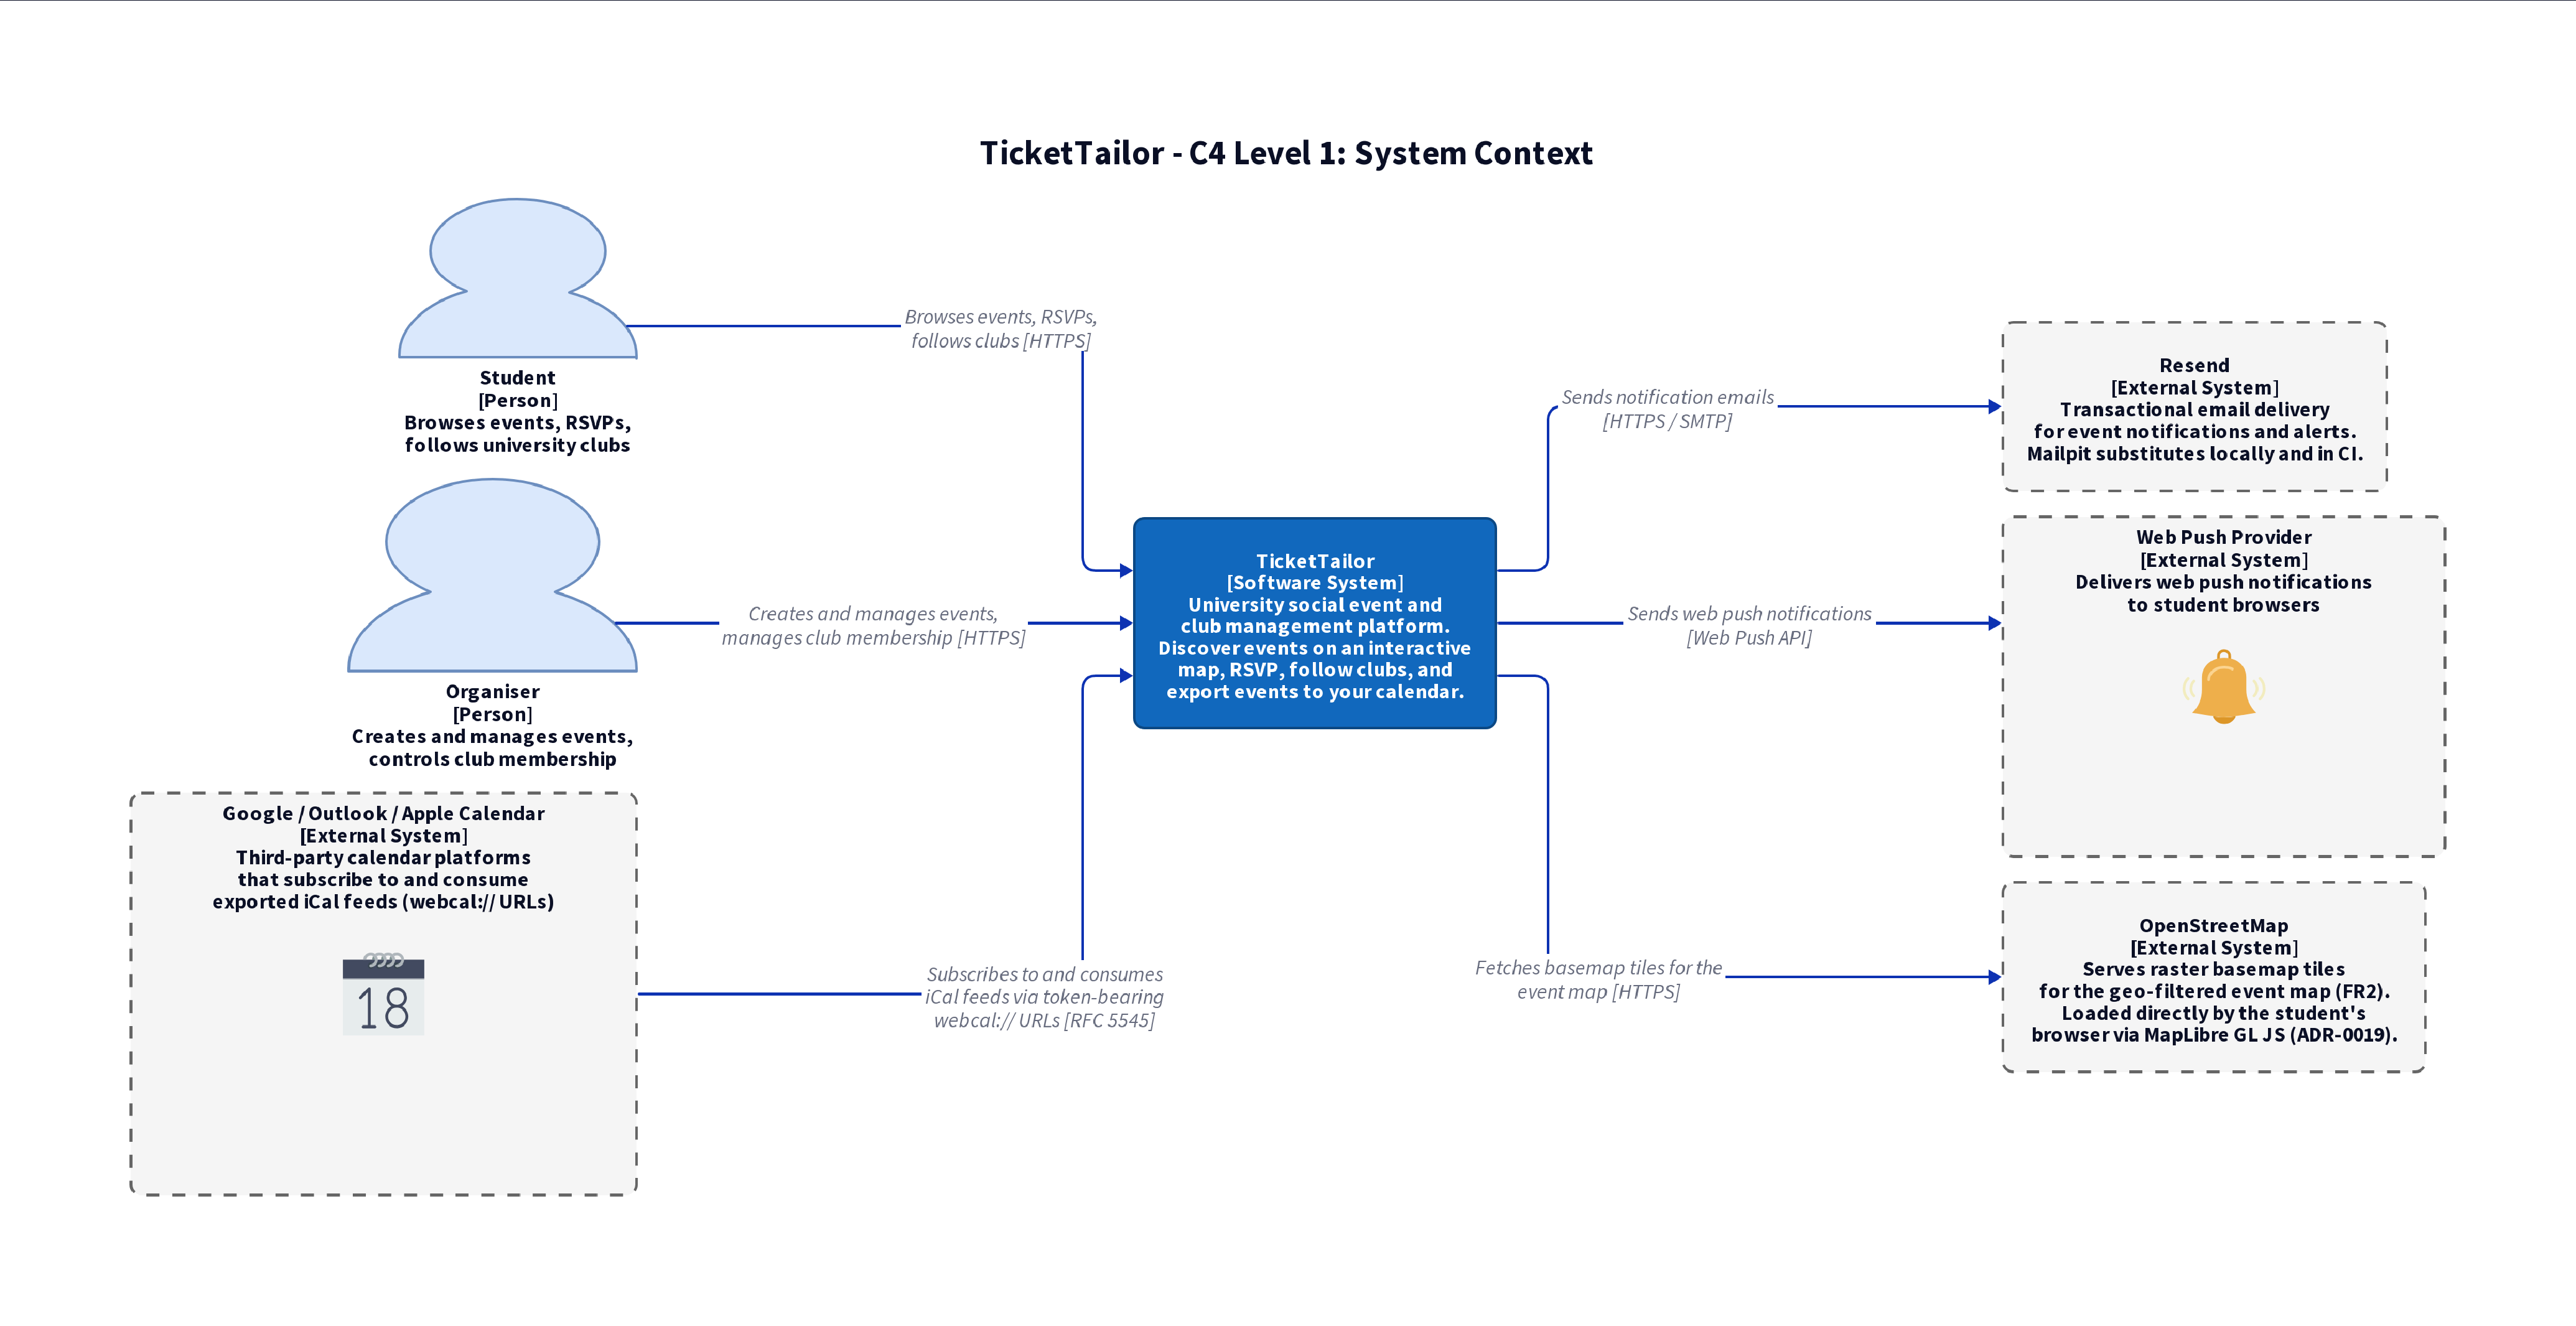
\includegraphics[width=\linewidth,height=0.82\textheight,keepaspectratio]{figures/c4_l1.pdf}
  \caption{C4 Level 1: system context. Students and committee members use one web client against a single public API, which integrates with four external services.}
  \label{fig:c4l1}
\end{figure}

Two human roles interact with TicketTailor. Students browse events on a geo-filtered map, RSVP, follow clubs, and receive notifications; committee members additionally create and manage events and configure pricing and visibility. Both use the same single-page web client, which talks to one public HTTP API.

The system integrates with four external services rather than re-implementing their concerns. Event details are exported as standards-compliant iCalendar feeds that any calendar client can consume (ADR-0007), so interoperability is achieved through an open format rather than per-vendor integrations. Real-time notifications are delivered through the browser's native Web Push service using VAPID (ADR-0011) and through an email provider, Resend (ADR-0012). Map tiles are loaded client-side directly from OpenStreetMap (ADR-0019), keeping tile traffic off the API entirely. Treating these as external systems keeps the core platform small and the trust boundary clear.

\subsection{Containers (C4 Level 2)}

\begin{figure}[htbp]
  \centering
  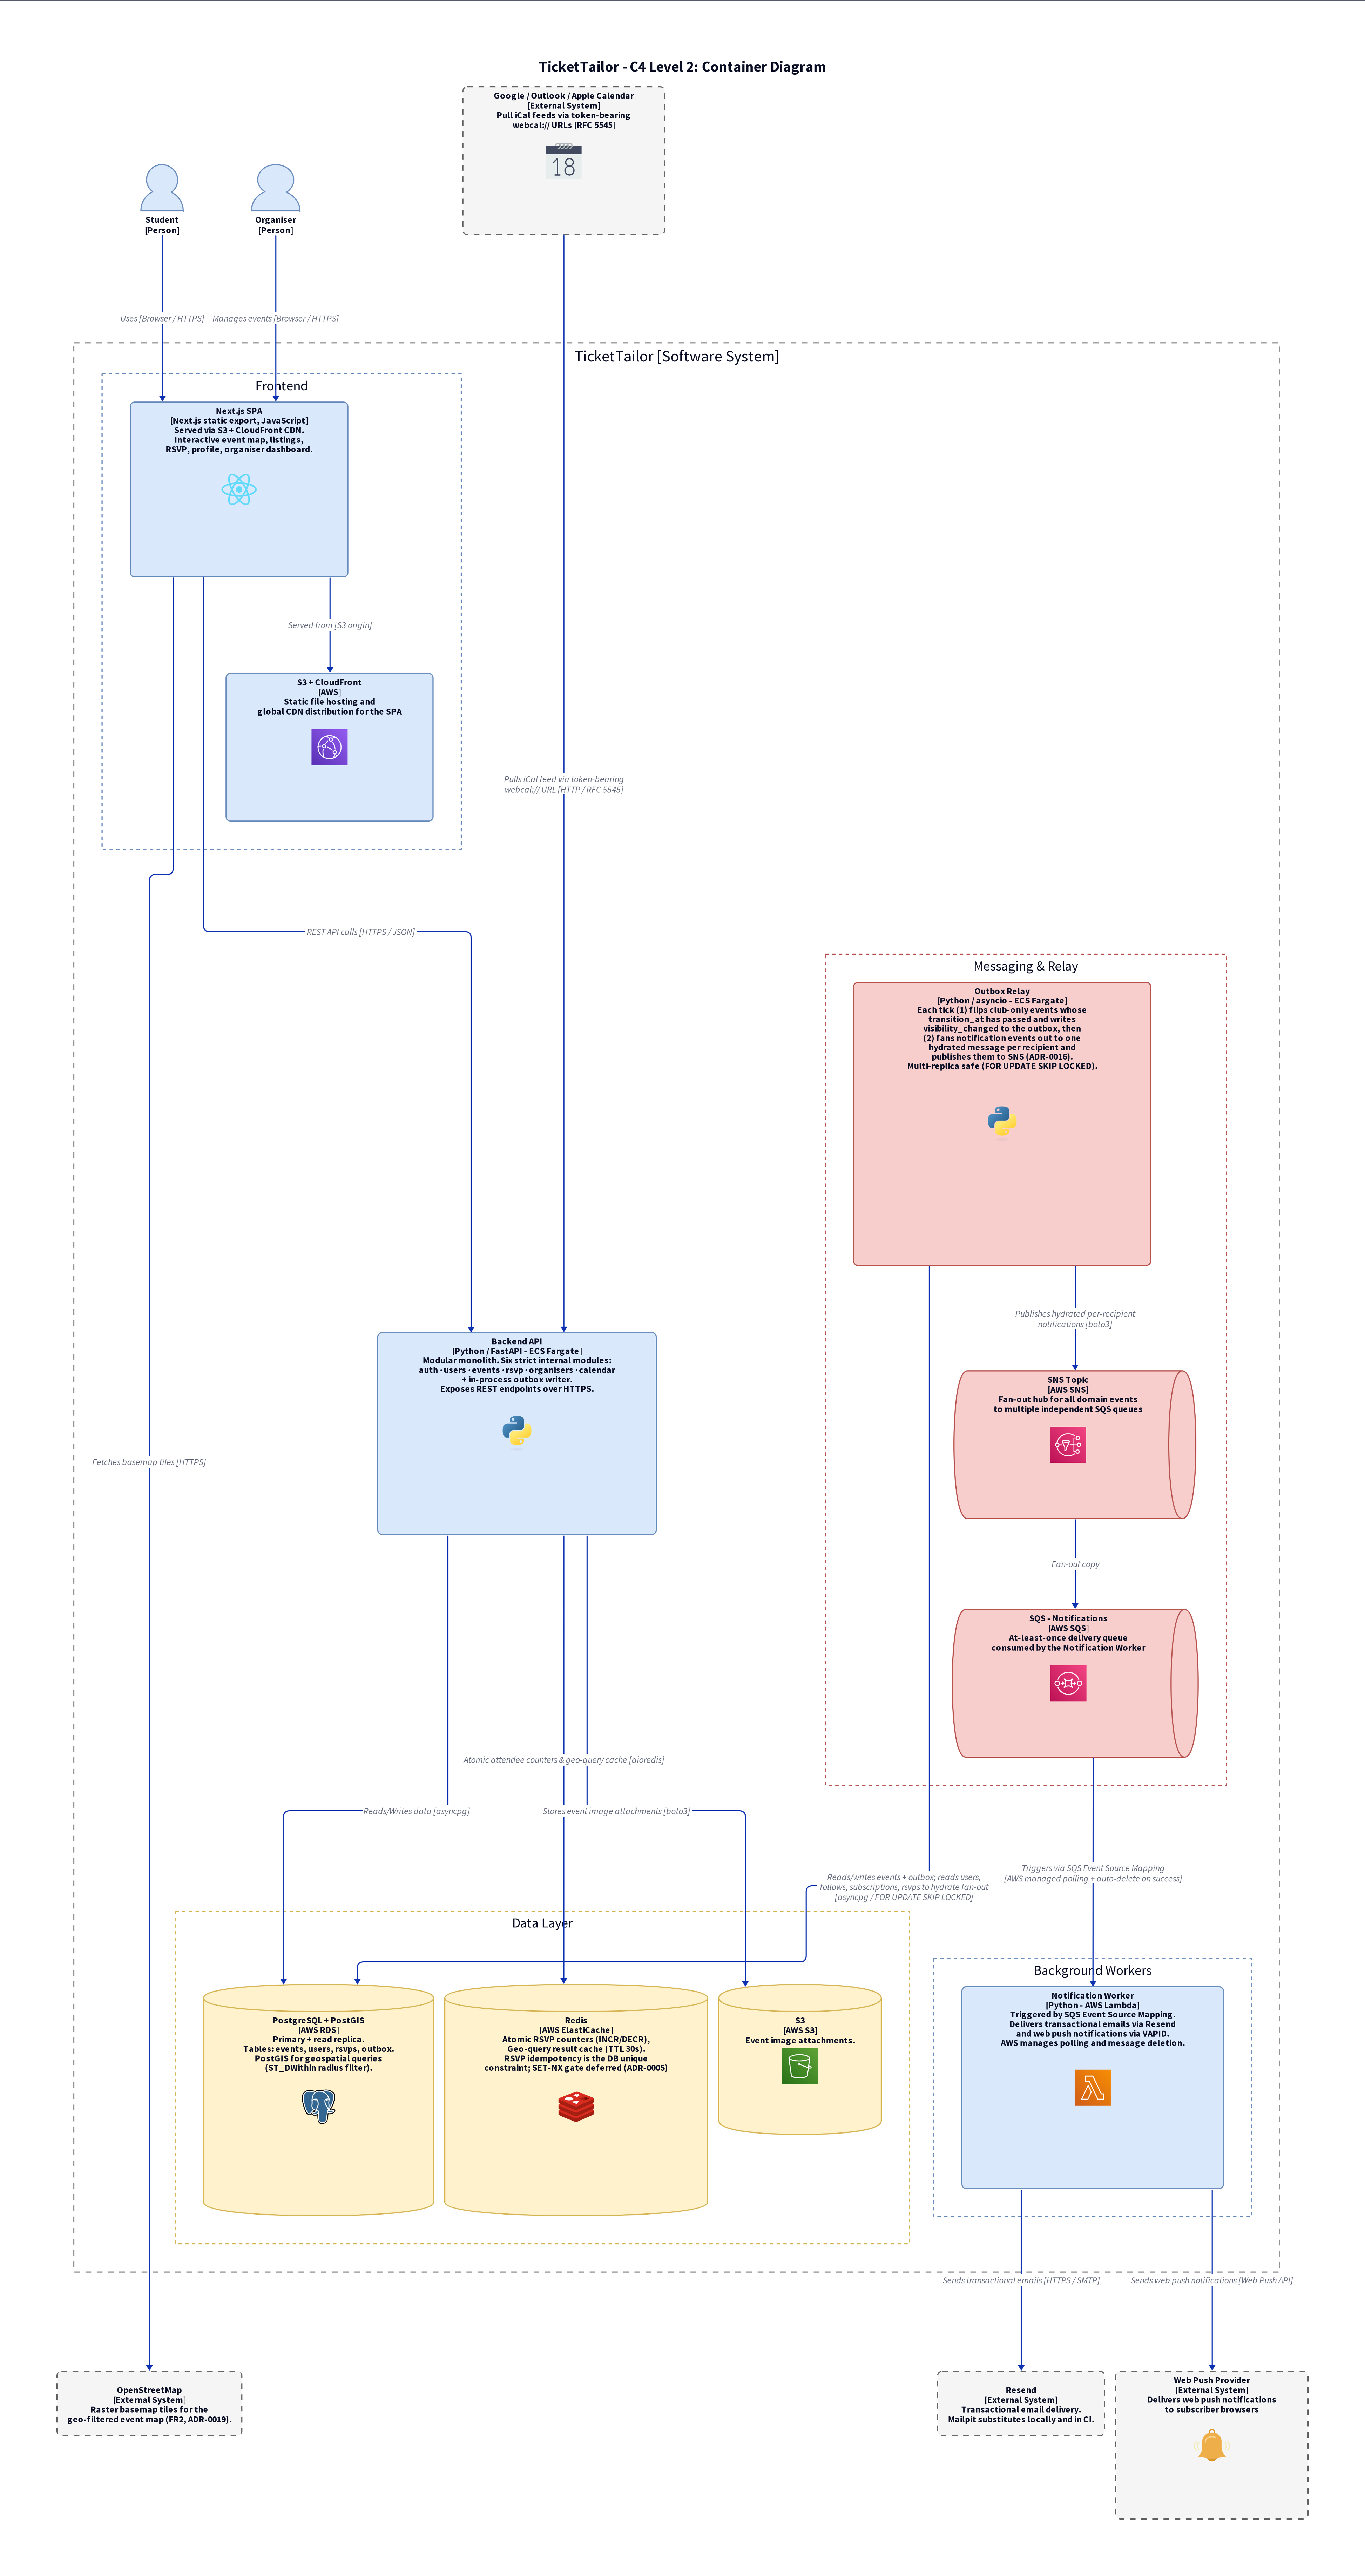
\includegraphics[width=\linewidth,height=0.82\textheight,keepaspectratio]{figures/c4_l2.pdf}
  \caption{C4 Level 2: containers. Three deployable backend units, three datastore concerns, and one static frontend.}
  \label{fig:c4l2}
\end{figure}

The platform comprises three independently deployable backend units, three datastore concerns, and one frontend, shown in Figure~\ref{fig:c4l2}.

The API is the modular monolith: a FastAPI application (ADR-0003) that handles all synchronous request and response traffic behind an application load balancer, and the only unit that accepts external requests. The outbox relay and the notification worker are extracted from the API precisely because their work is asynchronous and bursty and must not share the API's request path. The relay polls the transactional outbox, publishes domain events to the message bus, and additionally runs the scheduled FR5 visibility transition, the time-offset flip from club-only to public (ADR-0010). The worker consumes notification messages and performs the actual push and email delivery.

Three datastores back these units. A PostgreSQL primary with the PostGIS extension is the durable source of truth for relational data and geo-queries, with at least one read replica so that read-heavy map traffic does not contend with writes (ADR-0008). A Redis instance holds the live RSVP counter and short-lived caches, serving atomic \texttt{INCR} and \texttt{DECR} operations that would otherwise bottleneck on a single relational row (ADR-0005). An SNS topic fanned out to an SQS queue is the asynchronous boundary between the relay as publisher and the worker as consumer, with a dead-letter queue for messages that exhaust their retries (ADR-0006).

The frontend is a Next.js application compiled to a static bundle (ADR-0018); it holds no server-side logic and reaches the API over the same JSON contract as any other client. On the deployment target, the API and relay run as ECS Fargate services with independent auto-scaling, the worker runs as an AWS Lambda triggered by an SQS event-source mapping, and the datastores use managed equivalents (RDS, ElastiCache, SNS and SQS). The AWS Academy Learner Lab profile the project is actually deployed under is recorded in ADR-0017, with the static frontend served over HTTP from an S3 website on the lab (ADR-0020); neither substitution changes the container boundaries.

\subsection{Components: Inside the Modular Monolith (C4 Level 3)}

\begin{landscape}
\begin{figure}[htbp]
  \centering
  
\includegraphics[width=\linewidth,height=0.92\textwidth,keepaspectratio]{figures/c4_l3.pdf}
  \caption{C4 Level 3: components of the API container. Bounded domain modules over a shared infrastructure layer, each internally layered into router, service, and repository.}
  \label{fig:c4l3}
\end{figure}
\end{landscape}


Figure~\ref{fig:c4l3} opens the API container. It is partitioned into bounded domain modules for authentication, users, organisers, events, RSVP, and calendar, over a shared infrastructure layer. Each module is internally layered into a router for the HTTP surface, a service for business logic and authorisation, and a repository for persistence, which keeps authorisation logic testable in isolation rather than scattered through request handlers.

The decisive property is that these boundaries are enforced, not merely documented. Modules communicate only through one another's service interfaces; no module imports another's repositories or ORM models. The contract is checked mechanically in CI by import-linter (ADR-0002), so a boundary breach fails the build. Each module additionally owns its own database schema and migration history (ADR-0013), and cross-module needs are met through narrow, explicit seams: identity is supplied to every router by a single shared authentication dependency (ADR-0014), and cross-module invariants, such as confirming a club exists before a follow, are checked through registered shared callbacks rather than direct calls into another module's internals (ADR-0015). The result is a single deployable that is nonetheless decomposed cleanly enough that any module could later be extracted to its own service with a bounded, known change; that per-module extraction path is the project's answer to the expandable-to-a-larger-system criterion.

\subsection{Dominant Runtime Flow: Reliable Asynchronous Fan-out}

\begin{figure}[htbp]
  \centering
  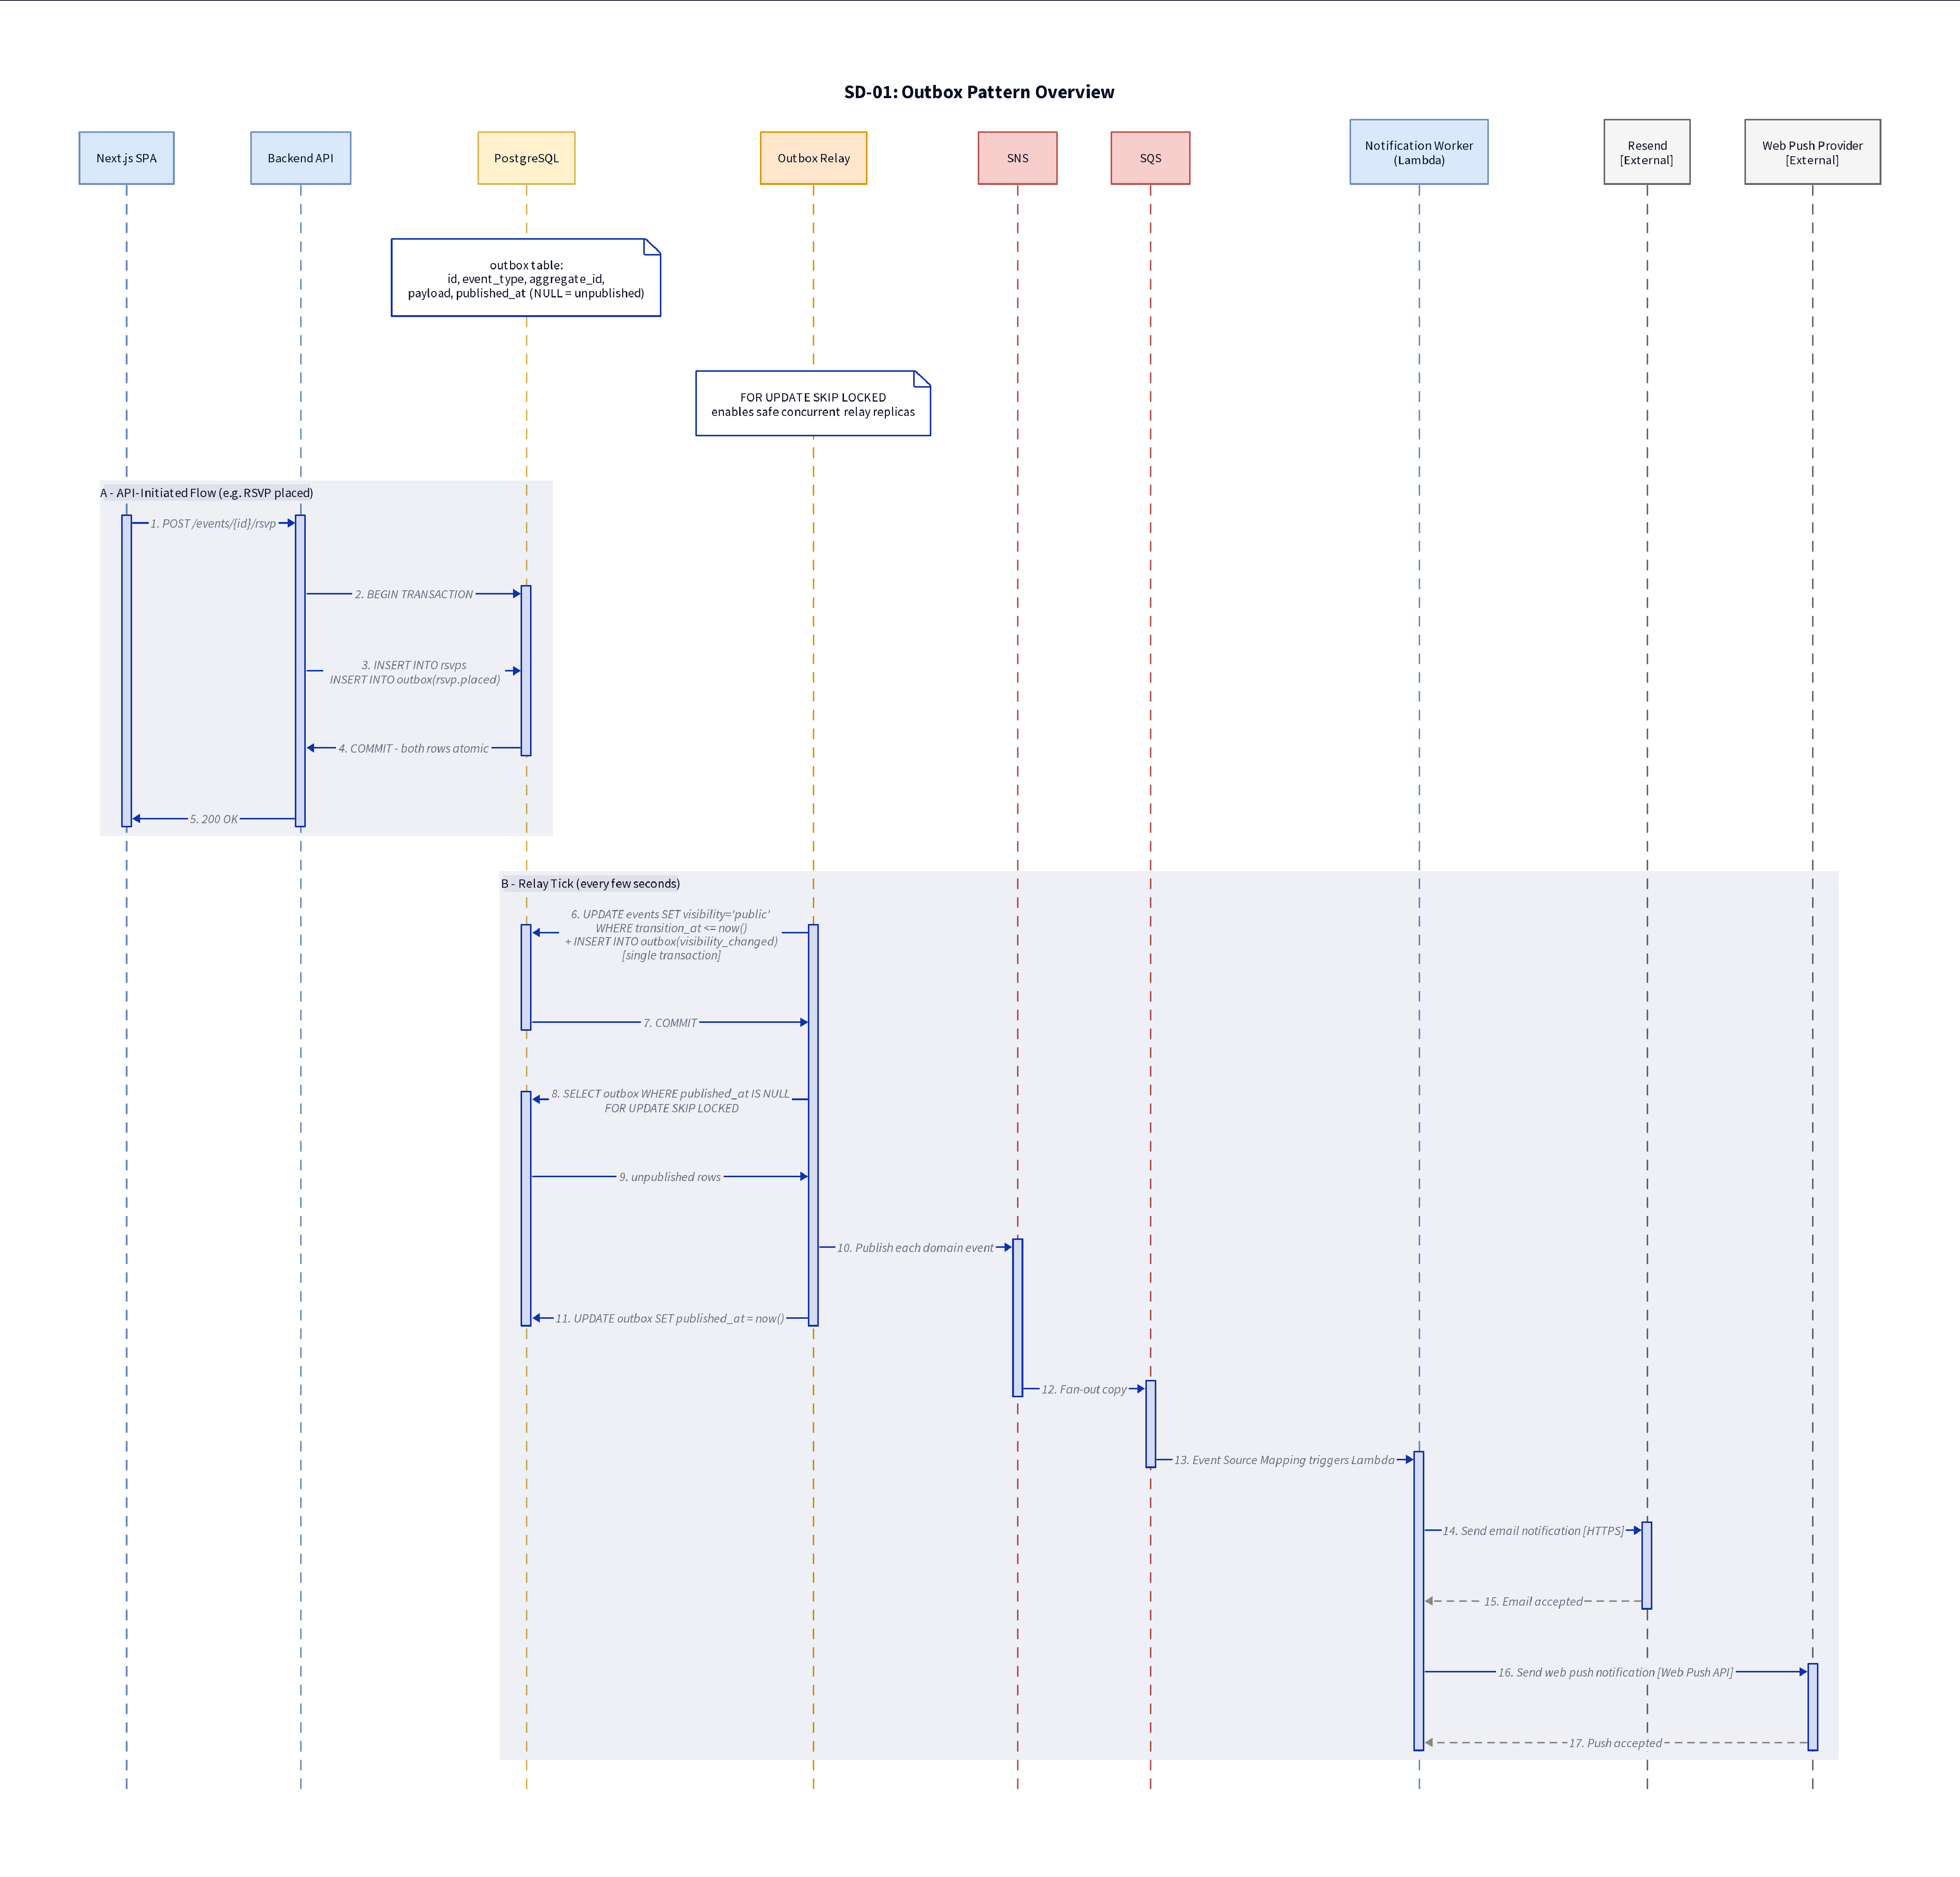
\includegraphics[width=\linewidth,height=0.78\textheight,keepaspectratio]{figures/seq_outbox.pdf}
  \caption{Outbox overview: a business write and its outbox row commit in one transaction; the relay publishes to SNS, which fans out to SQS and triggers the worker.}
  \label{fig:outbox}
\end{figure}

The architecture's most important dynamic behaviour is how a change inside the API reliably becomes a notification without coupling the two, traced in Figure~\ref{fig:outbox}. When a business write occurs, such as an RSVP, an organiser edit, or the visibility flip, the API commits the domain change and an outbox row in the same database transaction. Either both persist or neither does, so a request can never succeed while its notification event is silently lost. The relay then polls unpublished outbox rows, an index-backed scan that is proportional to the pending set rather than the whole table, and publishes each as a message to SNS. SNS fans the message out to the SQS queue, which triggers the worker. Because the relay hydrates each message with its recipient set before publishing (ADR-0016), the followers of the club for an FR5 transition or the RSVP'd attendees for an organiser edit, the worker delivers per recipient without reaching back into the database. Delivery is at-least-once: a transient failure is reported back to SQS so only the failed message is redelivered, and a message that exhausts its retries lands in the dead-letter queue rather than being dropped.

This single pattern carries much of the scalability and reliability story, set out in the next subsection.

\subsection{Satisfying the Architecturally Significant Requirements}

For scalability (QA1), the spike scenario, in which a popular event flips to public and notifies every follower while map traffic continues, is absorbed at four points. The notification worker is a separate process, so it scales as Lambda concurrency independently of the API; the SNS-to-SQS boundary decouples the rate of publishing from the rate of delivery, letting a backlog drain without back-pressuring the API; the read replica keeps the geo-query path off the write primary; and the Redis counter removes RSVP-count contention from a single database row. The headline load test delivered a fan-out to 300 followers in full with notification-ack p95 around 5 s, roughly six times under the 30 s target, and argues the 1{,}000-follower target by extrapolation, since ack latency stayed flat as the follower count grew (Section~\ref{sec:evaluation}).

For reliability (QA3), cross-replica correctness of attendee data is guaranteed by a combination of tactics, not replication alone. RSVP writes are idempotent through a unique constraint on \texttt{(user\_id, event\_id)}, so a retried or duplicated toggle cannot double-count. The transactional outbox makes cross-process events durable, as described above. A reconciliation job periodically compares the live Redis counter against the persisted RSVP rows and corrects any drift, and the at-least-once SQS delivery with a dead-letter queue ensures no notification is lost to a worker failure mid-fan-out. These are exercised directly by the reliability tests, including a primary-failover-mid-burst case (Section~\ref{sec:evaluation}).

For interoperability (QA2), the system emits RFC 5545 iCalendar feeds (ADR-0007) rather than integrating with each calendar vendor. A user saves an event once and the feed is consumed by Google, Outlook, or Apple Calendar; conformance is checked against an RFC 5545 validator and a manual round-trip. Choosing an open standard over vendor APIs keeps the surface small and avoids per-provider OAuth coupling, which is deferred as a stretch goal.

For security and privacy (QA4), authentication uses short-lived access tokens with rotating refresh tokens, and passwords are hashed with the memory-hard argon2id function (ADR-0009). Authorisation is role-based and lives in the service layer, so a student cannot mutate another club's events; ownership is checked through the organisers module rather than by trusting the request. Every request body is validated against a strict schema that rejects unknown fields, and the API's cross-origin policy is restricted to the deployed frontend origin. Transport is HTTPS in the idealised deployment; the Learner Lab's HTTP-only constraint and its mitigations are discussed in the critique (Section~\ref{sec:critique}).

Taken together, the structure keeps the common case simple, one cohesive API over one relational store, while isolating exactly the bursty, failure-prone notification path to which the quality attributes are most sensitive.